%%%%%%%%%%%%%%%%%%%%%%%%%%%%%%%%%%%%%%%%%%%%%%%%%%%%%%%%%%%%%%%%%%%%%%%%%%%%%%%
% Project: FAV 2009
% Authors:
%     Ondrej Lengal, xlenga00@stud.fit.vutbr.cz
%     Libor Polcak, xpolca03@stud.fit.vutbr.cz
%     Petr Zemek, xzemek02@stud.fit.vutbr.cz
%%%%%%%%%%%%%%%%%%%%%%%%%%%%%%%%%%%%%%%%%%%%%%%%%%%%%%%%%%%%%%%%%%%%%%%%%%%%%%%

\section*{Examples}
\label{sec:examples}

We decided to try some simple examples before implementation of our use-case problem (see Section \nameref{sec:use_case}). Two of these examples will be
presented here. Both of them originates from examples presented in our textbook\footnote{Mordechai Ben-Ari. \emph{Principles of the Spin Model Checker.} Springer, 2008.}, but we modified these examples according to our needs to grasp the basics of the Spin model checker and the underlying PROMELA language.

\subsection*{Non-deterministic finite automaton}

The first example shows a way how to obtain strings from a regular language accepted by some non-deterministic finite automaton (NFA). It was also our first example, where we learned the basics of the PROMELA language and Spin simulation capability.

\begin{lstlisting}[name=example1_listing]
inline GetRandomChar()
{
	if
	:: i = 'l';
	:: i = 'i';
	:: i = 'b';
	:: i = 'o';
	:: i = 'r';
	fi;
}
\end{lstlisting}

The \texttt{GetRandomChar()} ``procedure'' (PROMELA has only macros, which are specified by the \texttt{inline} word and work much like ANSI C macros) returns a random character from the set $\{l, i, b, o, r\}$. Random choice of a character is done by using an \texttt{if} statement, where every condition is \emph{executable} (it can be immediately evaluated to true). The chosen character is not returned --- it is set to variable \texttt{i}, which must be in scope when this macro is expanded.

\begin{figure}[h]
	\begin{center}
		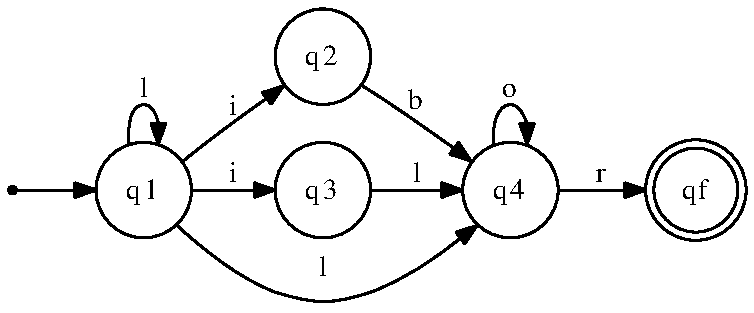
\includegraphics[width=9cm,keepaspectratio]{include/nfa}
	\end{center}
	\caption{State diagram of the implemented NFA.}
	\label{fig:NFA}
\end{figure}

The implementation of the NFA process follows (its state diagram is shown in Figure \ref{fig:NFA}).

\begin{lstlisting}[name=example1_listing]
active proctype NFA()
{
	byte i;

	GetRandomChar();

q1:
	if
	:: i == 'l' -> printf("l"); GetRandomChar(); goto q1;
	:: i == 'l' -> printf("l"); GetRandomChar(); goto q4;
	:: i == 'i' -> printf("i"); GetRandomChar(); goto q2;
	:: i == 'i' -> printf("i"); GetRandomChar(); goto q3;
	:: else -> GetRandomChar(); goto q1;
	fi;

q2:
	if
	:: i == 'b' -> printf("b"); GetRandomChar(); goto q4;
	:: else -> GetRandomChar(); goto q2;
	fi;

q3:
	if
	:: i == 'l' -> printf("l"); GetRandomChar(); goto q4;
	:: else -> GetRandomChar(); goto q3;
	fi;

q4:
	if
	:: i == 'o' -> printf("o"); GetRandomChar(); goto q4;
	:: i == 'r' -> printf("r"); GetRandomChar(); goto qf;
	:: else -> GetRandomChar(); goto q4;
	fi;

qf:
	printf("\n\nAccepted\n");
	assert (false);
}
\end{lstlisting}

The NFA is implemented in a \emph{label/goto} fashion. We use local variable \texttt{i} to store the current input symbol. At the beginning of the process, we obtain the first character and start in the starting state $q_{1}$. If the input symbol is from the set $\{l, i\}$, we print that character to the standard output and move to the proper state (again, non-determinism is present). Otherwise, we stay in the starting state and obtain another character (there was no transition with the previous character). We do this because we want to print a word accepted by the NFA, without getting stuck in some state from which there is no transition with the current input symbol.

The same principle as for the starting state is used for all other states. The string is accepted if we move from $q_{4}$ to the final state $q_{f}$. This situation is modelled by printing the \texttt{Accepted} string to standard output.

Sample output from 10 simulation runs:
\begin{verbatim}
iboor
lliboor
llibor
libor
iloor
lllr
lilr
libooor
ilr
llibr
\end{verbatim}

\subsection*{Channels}

Let us model the following situation. A \emph{client} can send a request and some of the available \emph{servers} will process it (thus modelling load balancing). After the processing finishes, the server sends a reply to the client, which awaits it as the answer to its request.

The second example utilizes \emph{message channels} to implement this client-server behaviour. A message channel can be viewed as a pipe, into which one side (a process) can send messages and some side (possibly the same process) can receive these messages. There are two types of message channels --- \emph{synchronous} (i.e., \emph{rendezvous}) and \emph{asynchronous} (i.e., \emph{buffered}). Synchronous channels do not have any buffer, so the sending side is blocked until there is a process that receives the message. Asynchronous channels contain a buffer of a specified length $n$, so if there are no more than $n-1$ messages in the channel, the message will be stored in the buffer and the sending side will not be blocked. From the point of view of the receiving side, if there are no messages in the channel, the receiving process is blocked until there is a message in the channel to be received.

The basic property that must hold in our system is that if a client sends a request, it eventually receives a reply from any of the servers. To check this property, we created the following LTL formula for each client $X$:

$$\Box(\mathrm{cXreq} \rightarrow \Diamond \mathrm{cXrep})$$

It precisely describes the needed property of our system --- it always holds that if a client $X$ sends a request ($cXreq$ is set to true), it eventually receives a reply ($cXrep$ is set to true). Using Spin, we can check that this formula holds in our system for all clients.

The implementation of our model follows:

\begin{lstlisting}[name=example2_listing]
// number of servers
#define SERVER_COUNT 2

// size of the request and response channel
#define REQ_CHAN_SIZE 4
#define REP_CHAN_SIZE 4

// number of values for each client counter
#define CNT_LEN 2
\end{lstlisting}

At the beginning of the source code, symbolic constants that are used in the implementation are defined. The syntax is the same as for the C programming language.

\begin{lstlisting}[name=example2_listing]
chan request = [REQ_CHAN_SIZE] of
{
	byte,        // client ID
	byte         // message num
};

chan reply = [REP_CHAN_SIZE] of
{
	byte,        // server ID
	byte,        // client ID
	byte         // message reply num
};
\end{lstlisting}

We will need two channels --- one for requests and one for replies. The \texttt{request} channel accepts and delivers pairs containing client ID and message sequence number. Client ID is used because we have only one channel for all clients, so client $X$ must accept only replies having this ID.

The \texttt{reply} channel accepts and delivers triples containing ID of the server which processed the request, client ID and message sequence number.

\begin{lstlisting}[name=example2_listing]
bool c1req = false;
bool c2req = false;
bool c3req = false;

bool c1rep = false;
bool c2rep = false;
bool c3rep = false;
\end{lstlisting}

These variables are used for verification based on checking properties described by LTL formulae. We model only three clients, because with more than three clients, the verifications ends with an \texttt{out of memory} error (tested on a 32-bit system without memory optimizations).

\begin{lstlisting}[name=example2_listing]
active [SERVER_COUNT] proctype Server()
{
	byte client;
	byte message;

end:
	do
	:: request ? client, message ->
		reply ! _pid, client, message;
		printf("Server %d processed request %d from client %d\n",
			_pid, message, client);
	od;
}
\end{lstlisting}

Each server is a standalone process which accepts messages from the \texttt{request} channel (line $36$) and replies to the \texttt{reply} channel (line $37$). After a request is processed, it prints an info message to the standard output (line $38$), which can be seen in a simulation. The \texttt{end} label is used to tell the verifier that the \texttt{do} loop is a valid termination point.

\begin{lstlisting}[name=example2_listing]
active proctype Client1()
{
	byte server;
	byte cnt;

	do
	:: cnt == CNT_LEN ->
		cnt = 0;
	:: else ->
		// clear flags
		c1req = false;
		c1rep = false;

		// send request
		request ! _pid, cnt;
		c1req = true;

		// receive reply
		reply ?? server, eval(_pid), eval(cnt);
		c1rep = true;

		// increment message sequence number
		cnt++;

		printf("Reply received by client %d from server %d\n", _pid, server);
	od;
}
\end{lstlisting}

Each client is also a standalone process. Because PROMELA does not contain every concept that can be found in popular modular programming languages, we had to create the same process for each client (the only difference is the client number).

Each client keeps a message sequence number counter, which is incremented after a reply is received. This number is used to distinguish between two consecutive replies.

In the main client process loop, if the message sequence number reaches its maximum (line $48$), it is set to zero to prevent overflow (line $49$). On lines $52$ and $53$, verification flags are set to false --- the process has neither sent a request nor received a reply. After a request is sent (line $56$), the \texttt{c1req} flag is set to true.

The process will then wait for the reply from any server (line $60$). Note that the PROMELA function \texttt{eval()} is used to turn process identification number \texttt{\_pid} and the message sequence number into constants, so that \emph{pattern matching} can be performed. This will cause the client to only receive its replies and not replies for other clients. When the reply is received, the \texttt{c1rep} is set to true (line $61$).

Finally, message sequence number counter is incremented (line $64$) and an info message is printed to the standard output.

%%%%%%%%%%%%%%%%%%%%%%%%%%%%%%%%%%%%%%%%%%%%%%%%%%%%%%%%%%%%%%%%%%%%%%%%%%%%%%%
% vim: syntax=tex
%%%%%%%%%%%%%%%%%%%%%%%%%%%%%%%%%%%%%%%%%%%%%%%%%%%%%%%%%%%%%%%%%%%%%%%%%%%%%%%
